\documentclass[tikz,border=6pt]{standalone}
\usepackage[T1]{fontenc}
\usepackage[scaled=0.92]{helvet}
\usepackage{amsmath,amssymb}
\usepackage{tikz}
\usetikzlibrary{arrows.meta,positioning,shapes.geometric,shapes.misc,calc,fit,backgrounds}

\begin{document}
\sffamily
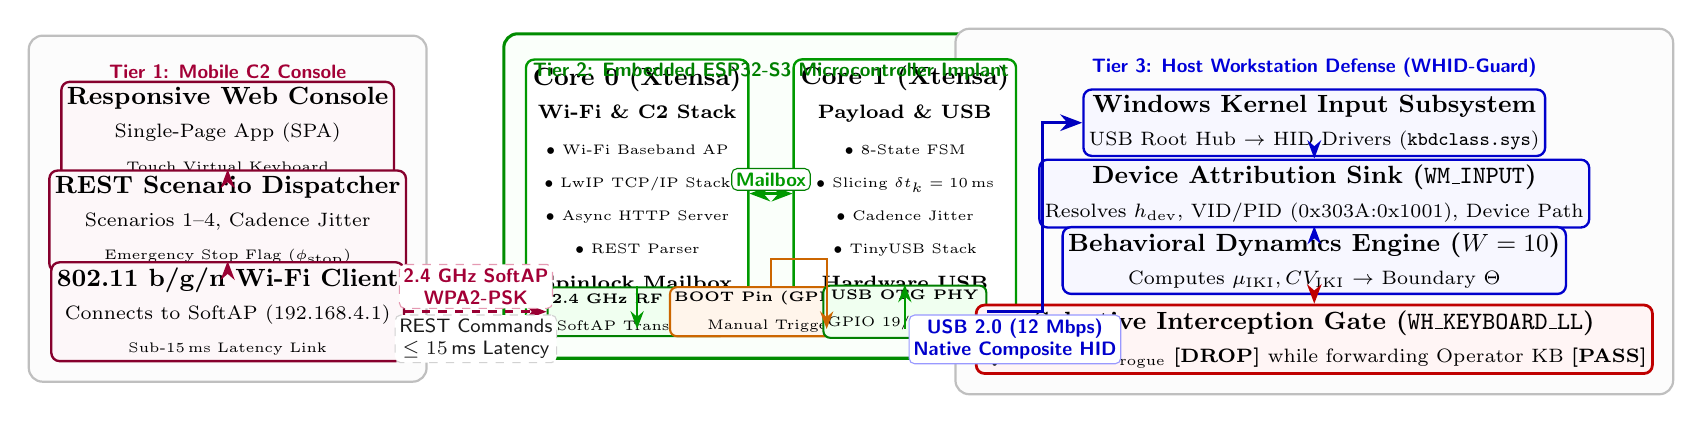
\begin{tikzpicture}[
    >=Stealth,
    font=\small,
    % Outer Container Styles
    tier_box/.style={
        rectangle,
        rounded corners=5pt,
        draw=gray!50,
        line width=0.8pt,
        fill=gray!2,
        inner sep=7pt
    },
    % Tier 1 Module Cards
    c2_card/.style={
        rectangle,
        rounded corners=3pt,
        draw=purple!70!black,
        line width=0.85pt,
        fill=purple!3!white,
        minimum width=3.3cm,
        minimum height=0.88cm,
        inner sep=2pt,
        align=center
    },
    % Tier 2 SoC Containers
    soc_chip/.style={
        rectangle,
        rounded corners=5pt,
        draw=green!55!black,
        line width=1.1pt,
        fill=green!2!white,
        inner sep=7pt
    },
    core_box/.style={
        rectangle,
        rounded corners=3pt,
        draw=green!60!black,
        line width=0.85pt,
        fill=white,
        minimum width=2.45cm,
        minimum height=2.15cm,
        inner sep=2.5pt,
        align=center
    },
    phy_box/.style={
        rectangle,
        rounded corners=2.5pt,
        draw=green!50!black,
        line width=0.75pt,
        fill=green!6!white,
        minimum width=1.55cm,
        minimum height=0.62cm,
        inner sep=1.5pt,
        align=center
    },
    % Tier 3 Host Cards
    host_card/.style={
        rectangle,
        rounded corners=3pt,
        draw=blue!80!black,
        line width=0.85pt,
        fill=blue!3!white,
        minimum width=4.6cm,
        minimum height=0.70cm,
        inner sep=2pt,
        align=center
    },
    gate_card/.style={
        rectangle,
        rounded corners=3pt,
        draw=red!75!black,
        line width=1.0pt,
        fill=red!4!white,
        minimum width=4.6cm,
        minimum height=0.72cm,
        inner sep=2pt,
        align=center
    },
    % Badges
    lbl/.style={
        font=\sffamily\scriptsize,
        fill=white,
        draw=gray!35,
        line width=0.4pt,
        rounded corners=2pt,
        inner sep=1.5pt,
        align=center,
        text=black!90
    },
    lbl_purple/.style={
        font=\sffamily\scriptsize\bfseries,
        fill=white,
        draw=purple!40,
        line width=0.4pt,
        rounded corners=2pt,
        inner sep=1.5pt,
        align=center,
        text=purple!85!black
    },
    lbl_green/.style={
        font=\sffamily\scriptsize\bfseries,
        fill=white,
        draw=green!50!black,
        line width=0.4pt,
        rounded corners=2pt,
        inner sep=1.5pt,
        align=center,
        text=green!60!black
    },
    lbl_blue/.style={
        font=\sffamily\scriptsize\bfseries,
        fill=white,
        draw=blue!40,
        line width=0.4pt,
        rounded corners=2pt,
        inner sep=1.5pt,
        align=center,
        text=blue!80!black
    }
]

% ==============================================================================
% TIER 1: Out-of-Band Mobile C2 Controller (x = 1.8)
% ==============================================================================
\node[c2_card] (c2_web)  at (1.8, 1.05) {\textbf{Responsive Web Console}\\[1pt]\scriptsize Single-Page App (SPA)\\[1pt]\tiny Touch Virtual Keyboard};
\node[c2_card] (c2_api)  at (1.8, -0.10) {\textbf{REST Scenario Dispatcher}\\[1pt]\scriptsize Scenarios 1--4, Cadence Jitter\\[1pt]\tiny Emergency Stop Flag ($\phi_{\text{stop}}$)};
\node[c2_card] (c2_wifi) at (1.8, -1.25) {\textbf{802.11 b/g/n Wi-Fi Client}\\[1pt]\scriptsize Connects to SoftAP ($192.168.4.1$)\\[1pt]\tiny Sub-15\,ms Latency Link};

\draw[->, line width=0.85pt, draw=purple!80!black] (c2_web.south) -- (c2_api.north);
\draw[->, line width=0.85pt, draw=purple!80!black] (c2_api.south) -- (c2_wifi.north);

\node[font=\sffamily\bfseries\scriptsize, text=purple!85!black] (t1_title) at (1.8, 1.80) {Tier 1: Mobile C2 Console};

\begin{scope}[on background layer]
    \node[tier_box, fit=(t1_title) (c2_web) (c2_api) (c2_wifi)] (tier1_bg) {};
\end{scope}

% ==============================================================================
% TIER 2: Embedded ESP32-S3 Hardware Implant (x = 7.0 to 10.6)
% ==============================================================================
% Core 0 Box (Wi-Fi Protocol Engine)
\node[core_box] (core0) at (7.0, 0.25) {
    \textbf{Core 0 (Xtensa)}\\[1pt]\scriptsize \textbf{Wi-Fi \& C2 Stack}\\[2pt]
    \tiny $\bullet$ Wi-Fi Baseband AP\\[1pt]
    \tiny $\bullet$ LwIP TCP/IP Stack\\[1pt]
    \tiny $\bullet$ Async HTTP Server\\[1pt]
    \tiny $\bullet$ REST Parser\\[2pt]
    \scriptsize \textbf{Spinlock Mailbox}\\[-1pt]
    \tiny \texttt{portMUX\_TYPE}
};

% Core 1 Box (Payload & USB FSM)
\node[core_box] (core1) at (10.4, 0.25) {
    \textbf{Core 1 (Xtensa)}\\[1pt]\scriptsize \textbf{Payload \& USB}\\[2pt]
    \tiny $\bullet$ 8-State FSM\\[1pt]
    \tiny $\bullet$ Slicing $\delta t_k=10$\,ms\\[1pt]
    \tiny $\bullet$ Cadence Jitter\\[1pt]
    \tiny $\bullet$ TinyUSB Stack\\[2pt]
    \scriptsize \textbf{Hardware USB}\\[-1pt]
    \tiny Direct D+/D- Pins
};

% Spinlock communication between cores
\draw[<->, line width=1.0pt, draw=green!60!black] (core0.east) -- node[above=1pt, lbl_green] {Mailbox} (core1.west);

% Integrated Hardware Peripheral Strip (Symmetric along bottom of SoC)
\node[phy_box] (phy_rf)   at (7.0, -1.25)  {\tiny\textbf{2.4 GHz RF / Ant}\\[-1pt]\tiny SoftAP Transceiver};
\node[phy_box, draw=orange!80!black, fill=orange!8!white] (phy_boot) at (8.7, -1.25)  {\tiny\textbf{BOOT Pin (GPIO 0)}\\[-1pt]\tiny Manual Trigger};
\node[phy_box] (phy_usb)  at (10.4, -1.25) {\tiny\textbf{USB OTG PHY}\\[-1pt]\tiny GPIO 19/20 ($D_\pm$)};

% Intra-chip vertical interconnects
\draw[->, line width=0.75pt, draw=green!60!black] (phy_rf.north) -- (core0.south);
\draw[->, line width=0.75pt, draw=orange!80!black] (phy_boot.north) -- ++(0, 0.35) -| (core1.240);
\draw[->, line width=0.75pt, draw=green!60!black] (core1.south) -- (phy_usb.north);

\node[font=\sffamily\bfseries\scriptsize, text=green!50!black] (t2_title) at (8.7, 1.80) {Tier 2: Embedded ESP32-S3 Microcontroller Implant};

\begin{scope}[on background layer]
    \node[soc_chip, fit=(t2_title) (core0) (core1) (phy_rf) (phy_boot) (phy_usb)] (soc_bg) {};
\end{scope}

% ==============================================================================
% RF Wireless Link (Tier 1 -> Tier 2) (From c2_wifi to phy_rf)
% ==============================================================================
\draw[->, line width=1.1pt, draw=purple!80!black, dashed] (c2_wifi.east) -- (phy_rf.west)
    node[pos=0.5, above=1pt, lbl_purple] {2.4 GHz SoftAP\\WPA2-PSK}
    node[pos=0.5, below=1pt, lbl] {REST Commands\\$\le 15$\,ms Latency};

% ==============================================================================
% TIER 3: Host Workstation & WHID-Guard Defense (x = 15.6)
% ==============================================================================
\node[host_card] (host_kernel) at (15.6, 1.15) {\textbf{Windows Kernel Input Subsystem}\\[1pt]\scriptsize USB Root Hub $\rightarrow$ HID Drivers (\texttt{kbdclass.sys})};

\node[host_card] (host_raw) at (15.6, 0.25) {\textbf{Device Attribution Sink (\texttt{WM\_INPUT})}\\[1pt]\scriptsize Resolves $h_{\text{dev}}$, VID/PID (0x303A:0x1001), Device Path};

\node[host_card] (host_engine) at (15.6, -0.60) {\textbf{Behavioral Dynamics Engine ($W=10$)}\\[1pt]\scriptsize Computes $\mu_{\text{IKI}}, CV_{\text{IKI}}$ $\rightarrow$ Boundary $\Theta$};

\node[gate_card] (host_gate) at (15.6, -1.60) {\textbf{Selective Interception Gate (\texttt{WH\_KEYBOARD\_LL})}\\[1pt]\scriptsize Quarantines $h_{\text{rogue}}$ \textbf{[DROP]} while forwarding Operator KB \textbf{[PASS]}};

% Host Internal Dataflows
\draw[->, line width=0.8pt, draw=blue!80!black] (host_kernel.south) -- (host_raw.north);
\draw[->, line width=0.8pt, draw=blue!80!black] (host_raw.south) -- (host_engine.north);
\draw[->, line width=0.9pt, draw=red!75!black] (host_engine.south) -- (host_gate.north);

\node[font=\sffamily\bfseries\scriptsize, text=blue!85!black] (t3_title) at (15.6, 1.85) {Tier 3: Host Workstation Defense (WHID-Guard)};

\begin{scope}[on background layer]
    \node[tier_box, fit=(t3_title) (host_kernel) (host_raw) (host_engine) (host_gate)] (tier3_bg) {};
\end{scope}

% ==============================================================================
% Physical USB 2.0 Differential Bus Link (Tier 2 -> Tier 3)
% Clean routing from phy_usb to host_kernel
% ==============================================================================
\draw[->, line width=1.1pt, draw=blue!75!black] (phy_usb.east) -- ++(0.7, 0)
    node[pos=0.5, below=1pt, lbl_blue] {USB 2.0 (12 Mbps)\\Native Composite HID}
    |- (host_kernel.west);

\end{tikzpicture}
\end{document}
